% Instructions to change to html version:
% Comment out:
%  minipage, multicols,columnbreak, mathbf, hrule
% Replace all: \begin{minipage}% \end{minipage} %\begin{mulicols}  %\end{mulicols}  %\columnbreak %% \begin{framed} %\end{framed} %%\hrule
% Search for \mathbf
% Replace $$ with \[ and $ with \(
% Enclose graphics in figure environments and add captions
% Re-tag \df environments as sections, subsections, etc.
% Command Line Code to Create html version:
%First: pdflatex -shell-escape filename.tex                                   
%Second, for each figure: inkscape "filename-figure1.pdf" -o "filename-figure1.png"
% Third: htlatex filename.tex "ht5mjlatex.cfg, charset=utf-8" " -cunihtf -utf8"

\documentclass[10pt]{article}

%\usepackage{tikz, pgf,pgfplots,wasysym,array}
%\usepackage{wasysym,array}

\usepackage{amsmath,amssymb}

\ifdefined\HCode
  \def\pgfsysdriver{pgfsys-tex4ht-updated.def}
\fi 
%\ifdefined\HCode
%  \def\pgfsysdriver{pgfsys-dvisvgm4ht.def}
%\fi 
\usepackage{tikz}
\usetikzlibrary{calc,decorations.markings,arrows}
\usepackage{pgfplots}

\pgfplotsset{compat=1.12}
\usepackage{myexternalize}
\usetikzlibrary{calc,decorations.markings,arrows}
\usepackage{framed}
\usepackage[none]{hyphenat}

\input{../../../common/1336_header_test.tex}
\begin{document}

\everymath{\displaystyle}

\renewcommand{\myTitle}{MATH 1336: Calculus III}

\renewcommand{\mySubTitle}{Section 1.4: Area \& Arclength in Polar Coordinates}
%~\hfill Name: \underline{~~~~~~~~~~~~~~~~~~~~~~~~~~~~~~~~~~~~~~~~~~~~~~~}


\lectTitle{\vspace*{-.5in}\myTitle}{\vspace*{.1in}\mySubTitle \vspace*{-.25in}}


\setlength{\columnseprule}{0.4pt}
\setlength{\columnsep}{3em}

%\hspace*{-.8in}%\begin{minipage}{1.25\textwidth}
%\begin{framed}

\section*{Integral Calculus in Polar Coordinates:}




%\begin{minipage}{.4\textwidth}


\begin{center}
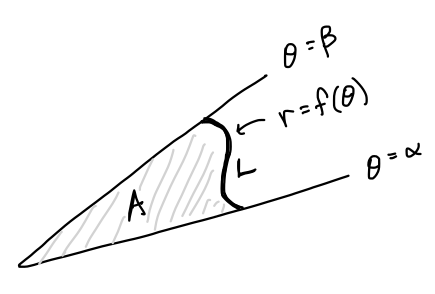
\includegraphics[height=2.in]{polar-area-arclength.png}

\vspace*{1in}

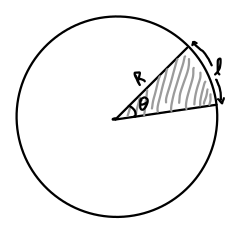
\includegraphics[height=1.5in]{circular-sector.png}
\end{center}

%\endminipage}
\hspace*{.2in}
%\begin{minipage}{.5\textwidth}










\subsection*{Area:}
The area enclosed by a polar curve from \(\theta = \alpha\) to \(\theta = \beta\) can be calculated using:
\[ A = \int_\alpha^\beta \frac{1}{2}r^2 \ d\theta \]

The key idea behind this formula is to break up the area into small sectors of circles, then add them up!\\~\\

\subsection*{Arclength:}

The arclength of polar curve from \(\theta = \alpha\) to \(\theta = \beta\) can be calculated using:
\[
 L= \int_{\alpha}^{\beta} \sqrt{r^2 + \left(\frac{dr}{d\theta}\right)^2}\ d\theta
\]

The key idea behind this formula is to break the curve up into small line segments, then add up the lengths of the line segments. Alternatively, it can be derived from the parametric arclength formula by using \(x = r\cos\theta,\  y = r\sin\theta\), and the product rule.\\~\\

\subsection*{Sectors of Circles:}

The derivations of the formulas above rely on geometric arguments involving the formulas for the area and length of an arc of a circular sector. For a circle of radius \(R\) and a sector with interior angle \(\theta\): 
\[
A_{\text{sector}} = \frac{1}{2}R^2\theta, \qquad \ell_{\textbf{sector}} = R\theta
\]
If you are interested, you can see the lecture notes for more details!\\

%\vspace*{-.2in}
%\endminipage}

%\end{framed}
%\endminipage}

%\begin{framed}
%\underline{\textbf{\Large Potentially Useful Forumlas:}}\\~\\
%%\small
%Polar Area:
%\[
% A = \int_\alpha^\beta \frac{1}{2}r^2 \ d\theta
%\]
%Polar Arclength: 
%\[
% L= \int_{\alpha}^{\beta} \sqrt{r^2 + \left(\frac{dr}{d\theta}\right)^2}\ d\theta
%\]
%%
%%\vspace*{-.2in}
%\end{framed}

\section*{In-class Problems:}

\begin{enumerate}
\item \textbf{Example 2 from 1.4 Lecture Notes}\\
Consider the four-leaved rose, which is described by the polar equation shown below.
\[
r =  \cos 2 \theta
\]
%\begin{multicols}{2}

%\begin{minipage}{.4\textwidth}
%\hspace*{-.5in}
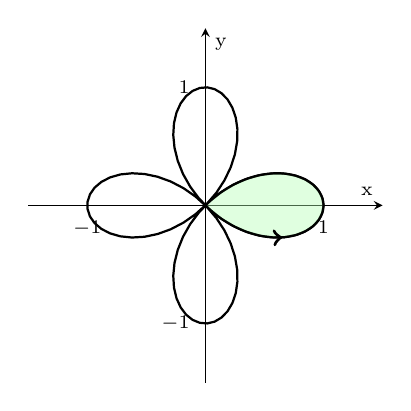
\begin{tikzpicture}
\begin{axis}[
	y=1.5cm,
    x=1.5cm,
	axis x line=middle,
	axis y line = middle,
	ymin=-1.5,ymax=1.5,
	xmin=-1.5,xmax=1.5,
    grid=none,
%    ticks=none,
%    yticklabels={},
%    xticklabels={},
    xtick={-1,...,1},
    ytick={-1,...,1},
    xlabel=x,
    ylabel=y,
    label style={font=\scriptsize},
    tick label style={font=\scriptsize}
]



\addplot[thick,black,variable=\t, domain=0:2*pi,samples=100,] ({(cos(2*deg(t)))*cos(deg(t))},{(cos(2*deg(t)))*sin(deg(t))});

\addplot[thick,black,variable=\t, domain=-pi/4:pi/4,samples=100,fill=green!30, fill opacity=.4,decoration = {markings,
    mark = at position .3 with {\arrow[line width=1.2pt]{>}}
  }, postaction = decorate] ({(cos(2*deg(t)))*cos(deg(t))},{(cos(2*deg(t)))*sin(deg(t))});
%\addplot+[black,only marks, mark=*, line width=2pt] coordinates{(5,0)(0,5)};
%\node [above] at (axis cs:  .15,.25) {\(C\)};

\end{axis}
%\filldraw[fill=green!20,draw=green!50!black] (1.5cm,0cm) -- (3.75cm,0cm) arc
%(0:45:3.75cm) -- (1.065cm,1.065cm) arc (45:0:1.5cm) -- cycle;
%
%

\end{tikzpicture}
%\endminipage}

%\columnbreakl
\begin{enumerate}
\item Set up and evaluate a definite integral to calculate the shaded area of one ``petal'' of the four-leaved rose, which is generated by \( -\frac{\pi}{4} \leq \theta \leq \frac{\pi}{4} \)\\
\item Set up \textbf{BUT DO NOT EVALUATE} a definite integral to calculate the length of the curve surrounding the shaded area.

\end{enumerate}

%\end{multicols}

\vfill

\pagebreak

\item \textbf{Example 3 from 1.4 Lecture Notes}\\
Find the area inside the circle \(r=1\) and outside the cardioid \(r=1-\cos\theta\).

%\begin{multicols}{2}

%\begin{minipage}{.4\textwidth}
%\hspace*{-.5in}
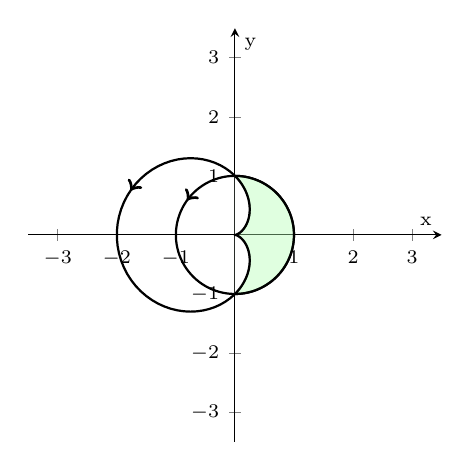
\begin{tikzpicture}
\begin{axis}[
	y=.75cm,
    x=.75cm,
	axis x line=middle,
	axis y line = middle,
	ymin=-3.5,ymax=3.5,
	xmin=-3.5,xmax=3.5,
    grid=none,
%    ticks=none,
%    yticklabels={},
%    xticklabels={},
    xtick={-3,-2,...,6},
    ytick={-5,-4,...,3},
    xlabel=x,
    ylabel=y,
    label style={font=\scriptsize},
    tick label style={font=\scriptsize}
]



\addplot[thick,black,variable=\t, domain=0:2*pi,samples=100,decoration = {markings,
    mark = at position .4 with {\arrow[line width=1.2pt]{>}}
  }, postaction = decorate] ({(1-cos(deg(t)))*cos(deg(t))},{(1-cos(deg(t)))*sin(deg(t))});

\addplot[thick,black,variable=\t, domain=0:2*pi,samples=100,decoration = {markings,
    mark = at position .4 with {\arrow[line width=1.2pt]{>}}
  }, postaction = decorate] ({cos(deg(t))},{sin(deg(t))});

\addplot[thick,black,variable=\t, domain=-pi/2:pi/2,samples=100,fill=green!30, fill opacity=.4] ({cos(deg(t))},{sin(deg(t))});
\addplot[thick,black,variable=\t, domain=-pi/2:pi/2, samples=100,fill=white, fill opacity=1,] ({(1-cos(deg(t)))*cos(deg(t))},{(1-cos(deg(t)))*sin(deg(t))});
%\addplot+[black,only marks, mark=*, line width=2pt] coordinates{(5,0)(0,5)};
%\node [above] at (axis cs:  .15,.25) {\(C\)};

\end{axis}
%\filldraw[fill=green!20,draw=green!50!black] (1.5cm,0cm) -- (3.75cm,0cm) arc
%(0:45:3.75cm) -- (1.065cm,1.065cm) arc (45:0:1.5cm) -- cycle;
%
%

\end{tikzpicture}
%\endminipage}

%\columnbreakl
\begin{enumerate}
\item Find the values of \(\theta\) where the curves intersect.
\item Use your answers from the previous part to help you set up a definite integral to calculate the shaded area.
\item Evaluate the integral you set up to calculate the shaded area.
\item Does the value you calculated for the area seem reasonable? Why or why not?

\end{enumerate}

%\end{multicols}

\vfill

\item Consider the curve described by the following polar equation, which is graphed on the axes below.
\[
r = 1 + \cos \theta
\]
%\begin{multicols}{2}

%\begin{minipage}{.4\textwidth}
%\hspace*{-.5in}
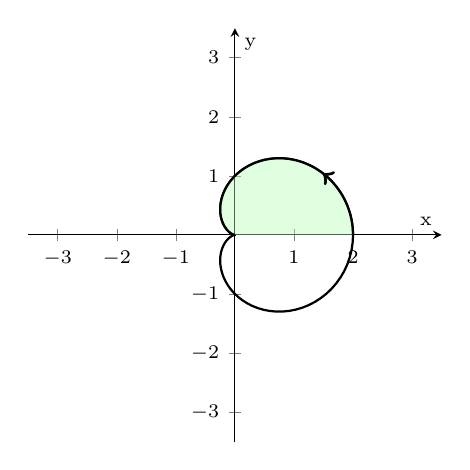
\begin{tikzpicture}
\begin{axis}[
	y=.75cm,
    x=.75cm,
	axis x line=middle,
	axis y line = middle,
	ymin=-3.5,ymax=3.5,
	xmin=-3.5,xmax=3.5,
    grid=none,
%    ticks=none,
%    yticklabels={},
%    xticklabels={},
    xtick={-3,-2,...,6},
    ytick={-5,-4,...,3},
    xlabel=x,
    ylabel=y,
    label style={font=\scriptsize},
    tick label style={font=\scriptsize}
]



\addplot[thick,black,variable=\t, domain=0:2*pi,samples=100,] ({(1+cos(deg(t)))*cos(deg(t))},{(1+cos(deg(t)))*sin(deg(t))});

\addplot[thick,black,variable=\t, domain=0:pi,samples=100,fill=green!30, fill opacity=.4,decoration = {markings,
    mark = at position .3 with {\arrow[line width=1.2pt]{>}}
  }, postaction = decorate] ({(1+cos(deg(t)))*cos(deg(t))},{(1+cos(deg(t)))*sin(deg(t))});
%\addplot+[black,only marks, mark=*, line width=2pt] coordinates{(5,0)(0,5)};
%\node [above] at (axis cs:  .15,.25) {\(C\)};

\end{axis}
%\filldraw[fill=green!20,draw=green!50!black] (1.5cm,0cm) -- (3.75cm,0cm) arc
%(0:45:3.75cm) -- (1.065cm,1.065cm) arc (45:0:1.5cm) -- cycle;
%
%

\end{tikzpicture}
%\endminipage}

%\columnbreakl
\begin{enumerate}
\item Set up and evaluate a definite integral to calculate the shaded area.
\item Use symmetry to calculate the entire enclosed area. Does your answer seem reasonable? Why or why not?
\item Set up \textbf{BUT DO NOT EVALUATE} a definite integral to calculate the length of the curve above the shaded area.

\end{enumerate}

%\end{multicols}

\vfill

\item Find the area of the region that is bounded by the given curve, and lies in the specified sector:
\[
r=e^{-\theta/4}, \qquad \pi/2\leq \theta \leq \pi
\]

\vfill

\item Find the exact length of the polar curve:
\[
r=e^{2\theta}, \qquad 0\leq \theta \leq 2\pi
\]

\vfill



\end{enumerate}

\end{document}
